\chapter{INITIAL OUTPUTS}
\thispagestyle{empty}

\section{Produced Artifacts}

The project has already produced a substantial set of concrete outputs rather
than only preliminary code fragments. The most important artifacts are:
\begin{itemize}
    \item the Custom-WikiCS experimental dataset derived from Wiki-CS with
    enriched Wikipedia text fields,
    \item semantic embedding caches based on BGE-M3,
    \item structural embedding caches for multiple Node2Vec variants,
    \item revised GCN and GraphSAGE training notebooks on the new branch,
    \item a ten-model evaluation branch with unified metrics,
    \item a working local web application prototype for article search,
    recommendation, and preview.
\end{itemize}

Figure~\ref{fig:architecture} summarizes the overall project pipeline. It
captures the three main stages that now structure the implementation:
data preparation, embedding generation, and recommendation/presentation.

\begin{figure}[H]
\centering
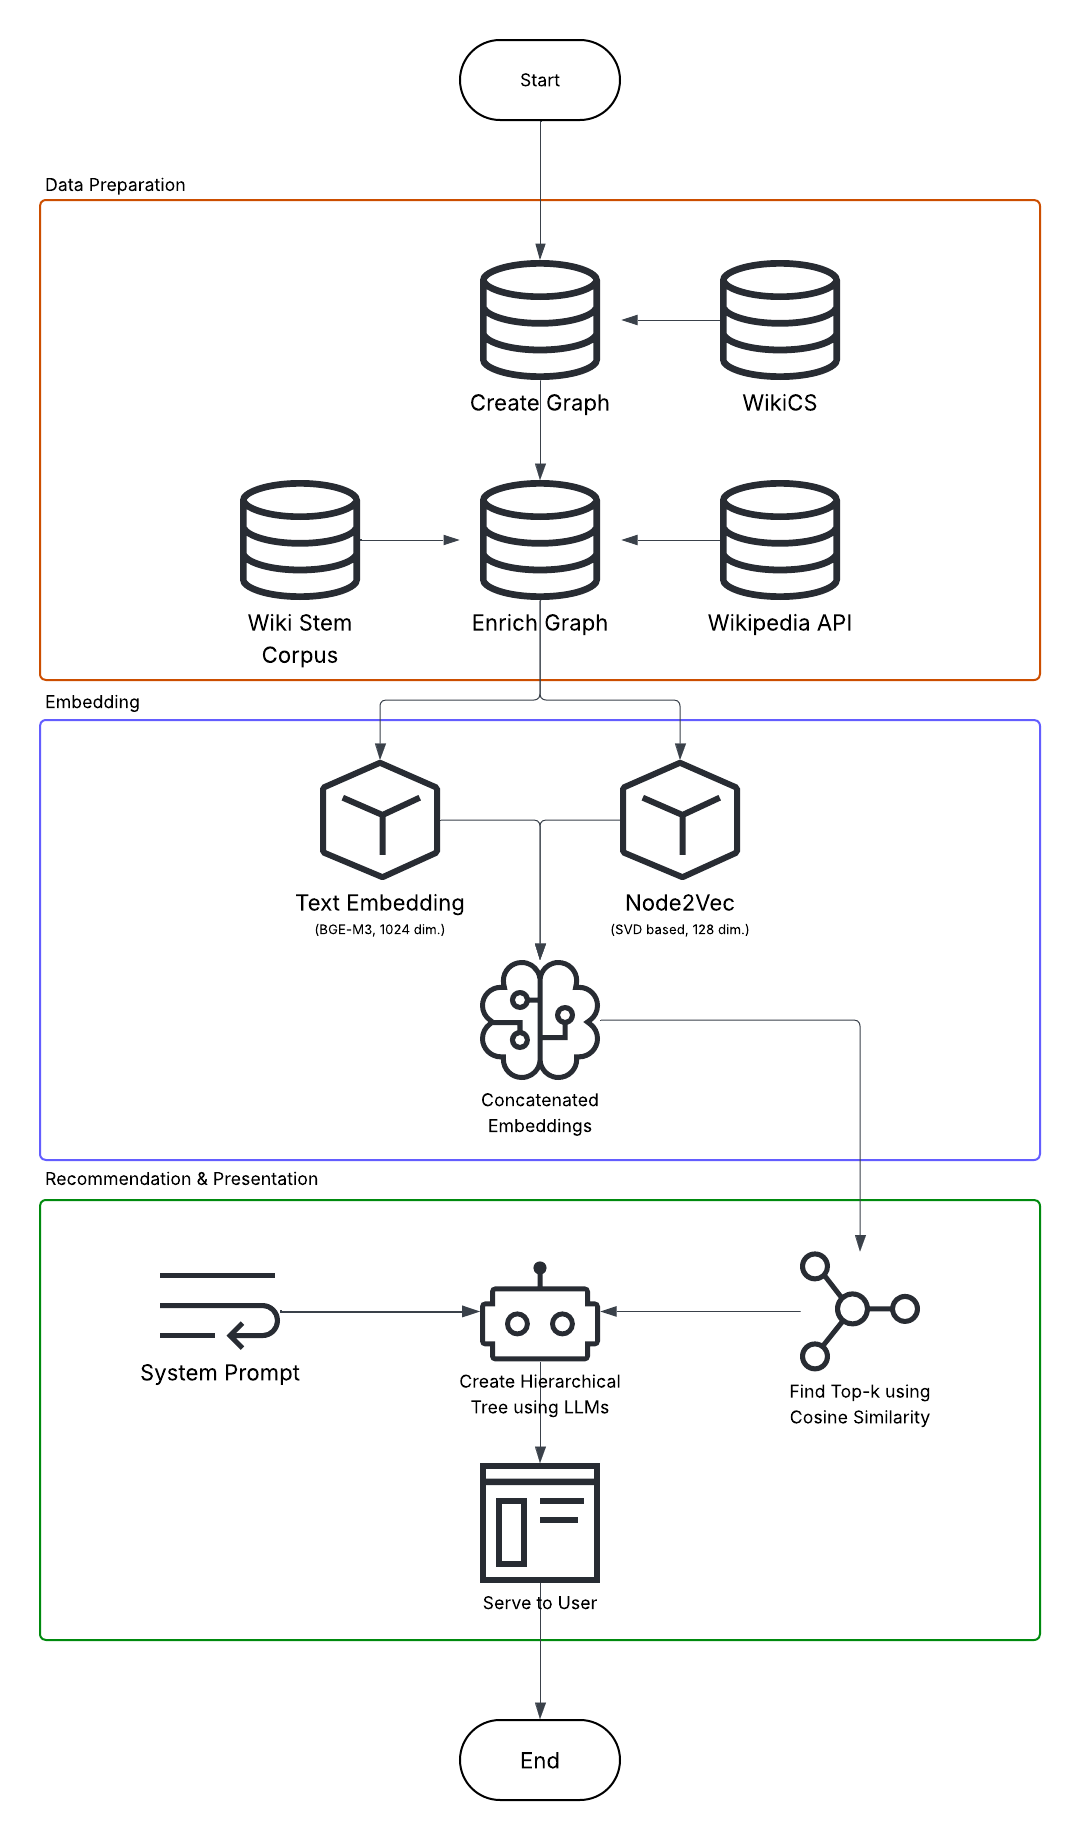
\includegraphics[width=0.88\textwidth]{figures/architecture.png}
\caption{Overall architecture of the project pipeline, from graph creation to recommendation and future learning-path presentation.}
\label{fig:architecture}
\end{figure}

The project also includes an interactive user-facing prototype. The current web
application supports live article search, model selection, ranked retrieval,
article preview, and an experimental learning-path view. The interface design
direction is illustrated in Figure~\ref{fig:mockup}; the implemented local
prototype now follows the same high-level idea, with search on the left,
recommendations in the center, and contextual detail on the right.

\begin{figure}[H]
\centering
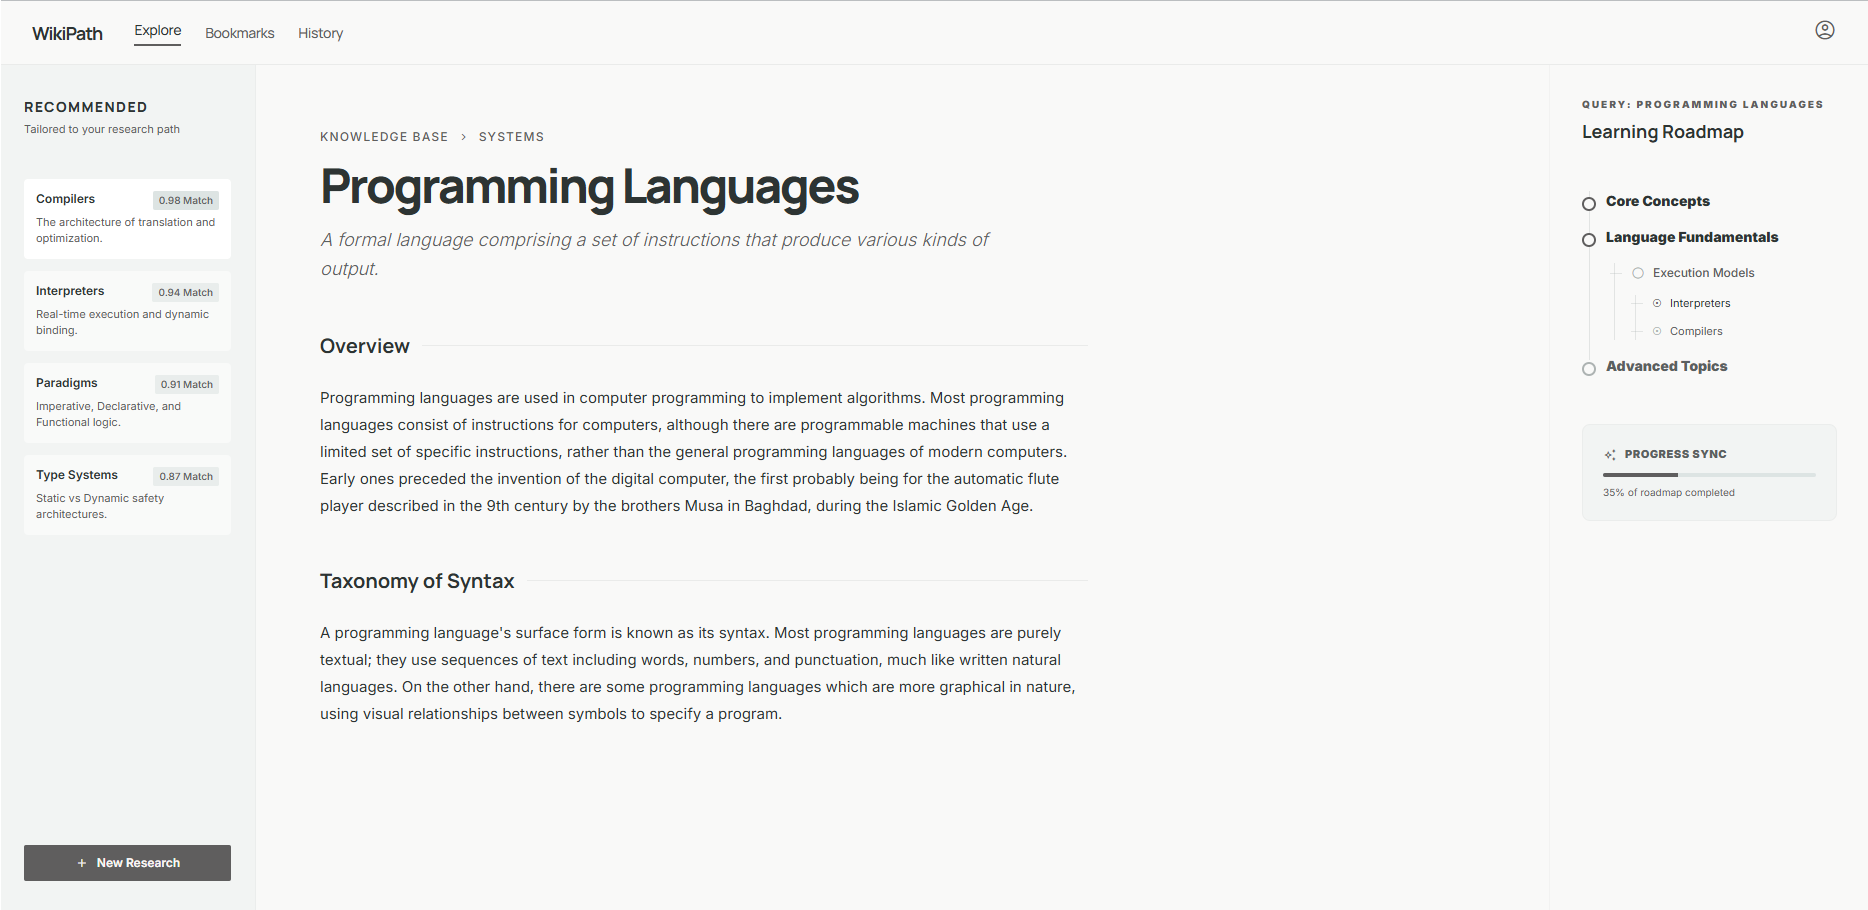
\includegraphics[width=\textwidth]{figures/interface-mockup.png}
\caption{Interface concept for the recommendation system, showing the move from flat retrieval toward structured learning-path presentation.}
\label{fig:mockup}
\end{figure}

The structural analysis outputs from earlier stages also remain relevant. The
degree distribution of the graph continues to exhibit a heavy-tailed behavior,
which motivated the popularity-aware correction experiments later used in the
Node2Vec family. This is illustrated again in
Figure~\ref{fig:degree-log-log}.

\begin{figure}[H]
\centering
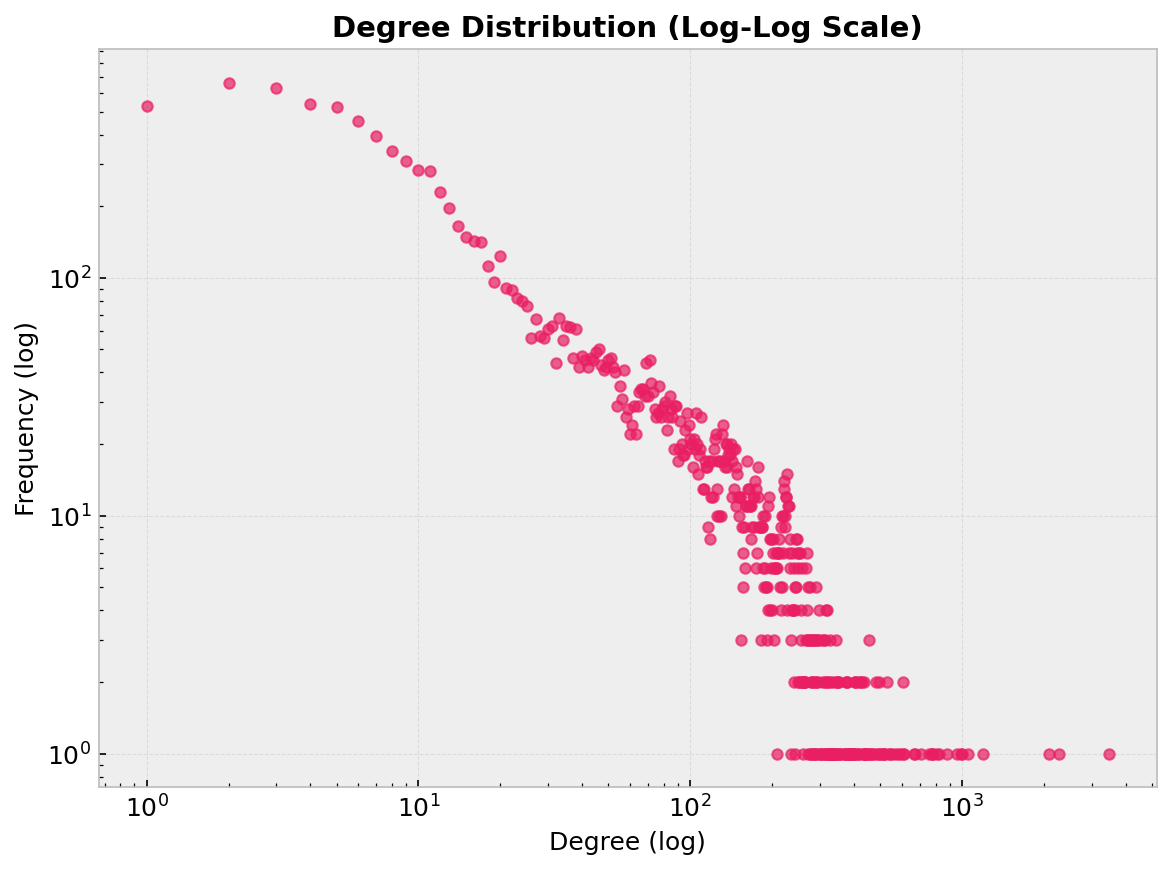
\includegraphics[width=0.78\textwidth]{figures/degree-log-log.png}
\caption{Log-log degree distribution of the Custom-WikiCS graph, showing the heavy-tailed structural behavior of the article network.}
\label{fig:degree-log-log}
\end{figure}

Beyond degree alone, earlier graph analysis also showed that node importance is
highly uneven across centrality families. Figure~\ref{fig:centrality} confirms
that degree, PageRank, betweenness, and eigenvector centralities are all
strongly skewed, reinforcing the need to monitor popularity effects in
recommendation experiments.

\begin{figure}[H]
\centering
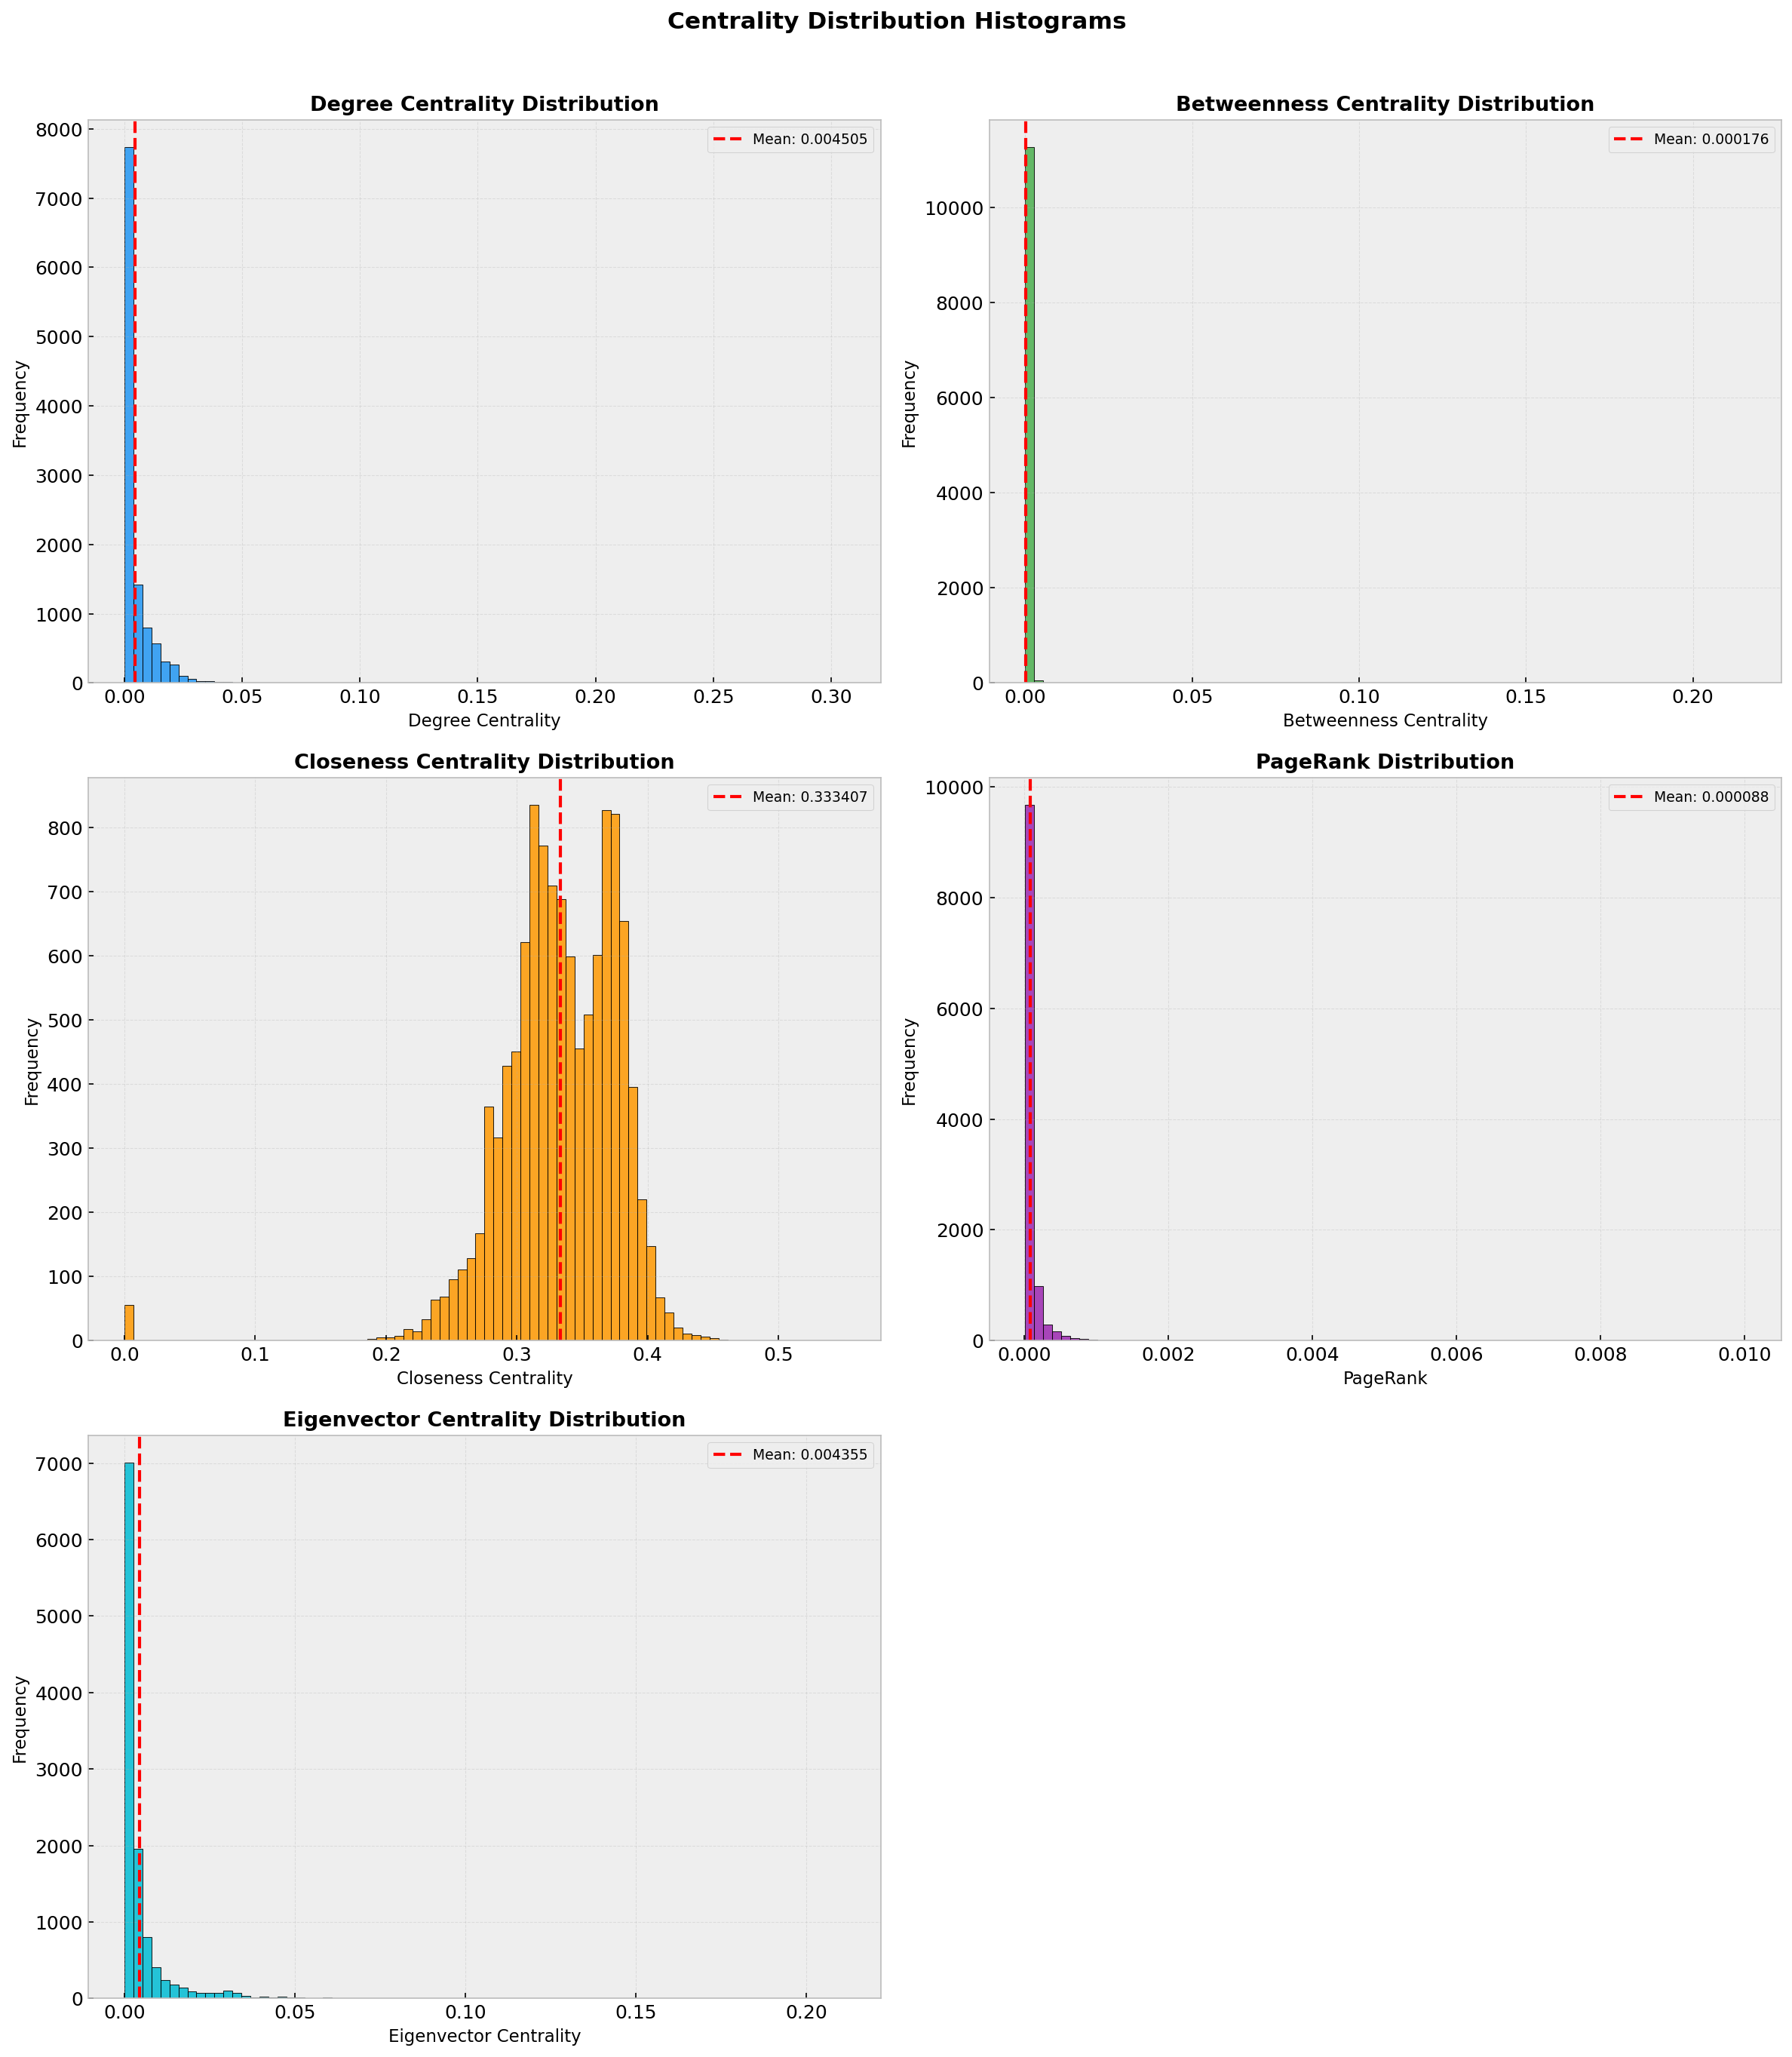
\includegraphics[width=0.88\textwidth]{figures/centrality-histograms.png}
\caption{Centrality distribution histograms from the Custom-WikiCS graph analysis. The strong skew across several centrality measures motivates popularity-aware evaluation.}
\label{fig:centrality}
\end{figure}

Community analysis also produced a meaningful structural output. The Louvain
partition shown in Figure~\ref{fig:louvain} indicates that the graph is not
uniformly mixed, but instead organized into communities of highly unequal size.
This supports the intuition that a recommendation model must balance local
topical neighborhoods against broader graph connectivity.

\begin{figure}[H]
\centering
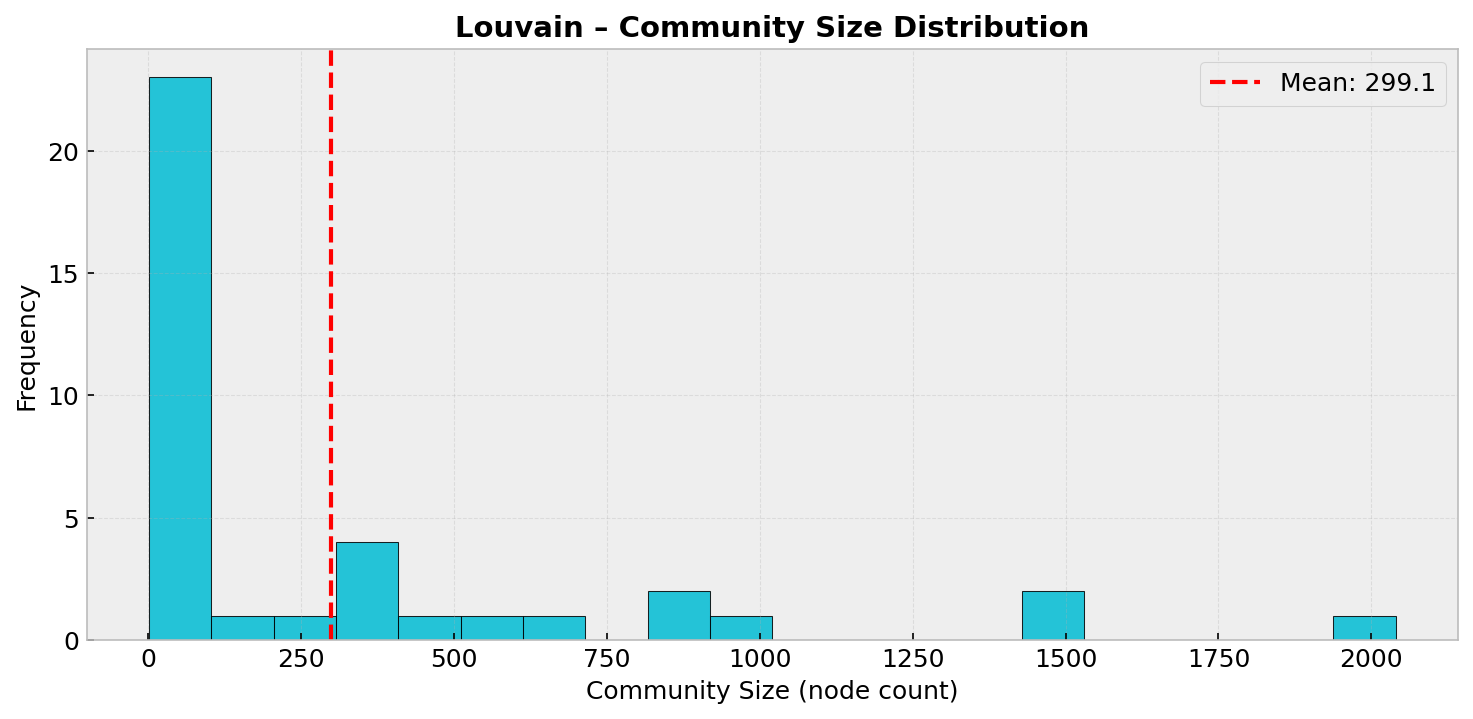
\includegraphics[width=0.82\textwidth]{figures/community-size-distribution-louvain.png}
\caption{Louvain community size distribution for the Custom-WikiCS graph. A few large communities coexist with many smaller ones, indicating non-uniform topic structure.}
\label{fig:louvain}
\end{figure}

\section{Current Experimental Results}

The most important current output is the revised evaluation branch built on an
undirected structural split. In that branch, the full graph is first converted
to an undirected graph and then split into 172,900 training edges and 43,223
test edges, producing 86,446 expanded evaluation pairs over 9,022 evaluation
nodes. This branch retrains the structural family and evaluates ten models in a
single comparison.

Table~\ref{tab:selected-results} presents a compact summary of the current
results. The strongest performance now comes from the corrected hybrid family,
not from pure structural retrieval alone.

\begin{table}[H]
\centering
\caption{Selected results from the revised ten-model evaluation branch.}
\label{tab:selected-results}
\begin{tabular}{p{0.38\textwidth}cccc}
\toprule
\textbf{Model} & \textbf{Hit@10} & \textbf{MRR} & \textbf{Pop. Lift} & \textbf{ILD} \\
\midrule
BGE pooled + Node2Vec (corrected) & 0.0867 & 0.0410 & 1.3301 & 0.4372 \\
BGE-M3 + Node2Vec (corrected) & 0.0867 & 0.0421 & 1.3081 & 0.4316 \\
Node2Vec (uncorrected) & 0.0781 & 0.0375 & 1.3374 & 0.4569 \\
Node2Vec (corrected) & 0.0781 & 0.0375 & 1.3374 & 0.4569 \\
GCN + BGE-M3 (rank fusion) & 0.0763 & 0.0335 & 1.6650 & 0.4366 \\
BGE-M3 Only & 0.0757 & 0.0366 & 1.9413 & 0.3713 \\
GCN Only & 0.0346 & 0.0180 & 1.1879 & 0.5135 \\
GraphSAGE Only & 0.0122 & 0.0076 & 1.3134 & 0.5313 \\
\bottomrule
\end{tabular}
\end{table}

These results already suggest two important conclusions. First, the older
impression that uncorrected Node2Vec clearly dominates the project no longer
holds under the revised branch. Second, the best-performing models are now the
semantic-structural hybrids, especially the corrected variants that combine
BGE-M3 with leakage-free structural information.
